\section{Application: Perspective rendering}

As an application of linear transformations, we consider the problem
of perspective rendering. Imagine some object has been described by
coordinates in 3-dimensional space, and we wish to make an image of
the object as it would be seen by a human eye or by a camera. The
process of computing such an image is known as \textbf{rendering}%
\index{rendering}.

Conceptually, the rendering process makes use of a \textbf{camera}%
\index{camera}, which we will assume is located at the origin of a
3-dimensional coordinate system called the \textbf{camera coordinate
  system}%
\index{camera coordinates}%
\index{coordinate system!camera coordinates}, and an \textbf{image
  plane}%
\index{image plane}%
\index{plane!image plane}, which we will assume is the plane $z=1$ in
camera coordinates. The 3-dimensional space also contains one or more
objects that we wish to render. We can consider the object to be
described by a set of points. For each point $\vect{p}$ on the object,
draw a straight line from $\vect{p}$ to the camera, and let
$\vect{p}'$ be the point where this line intersects the image
plane. The point $\vect{p}$ of the object is rendered as the point
$\vect{p}'$ in the image. This process is illustrated in the following
figure:
\begin{equation*}
  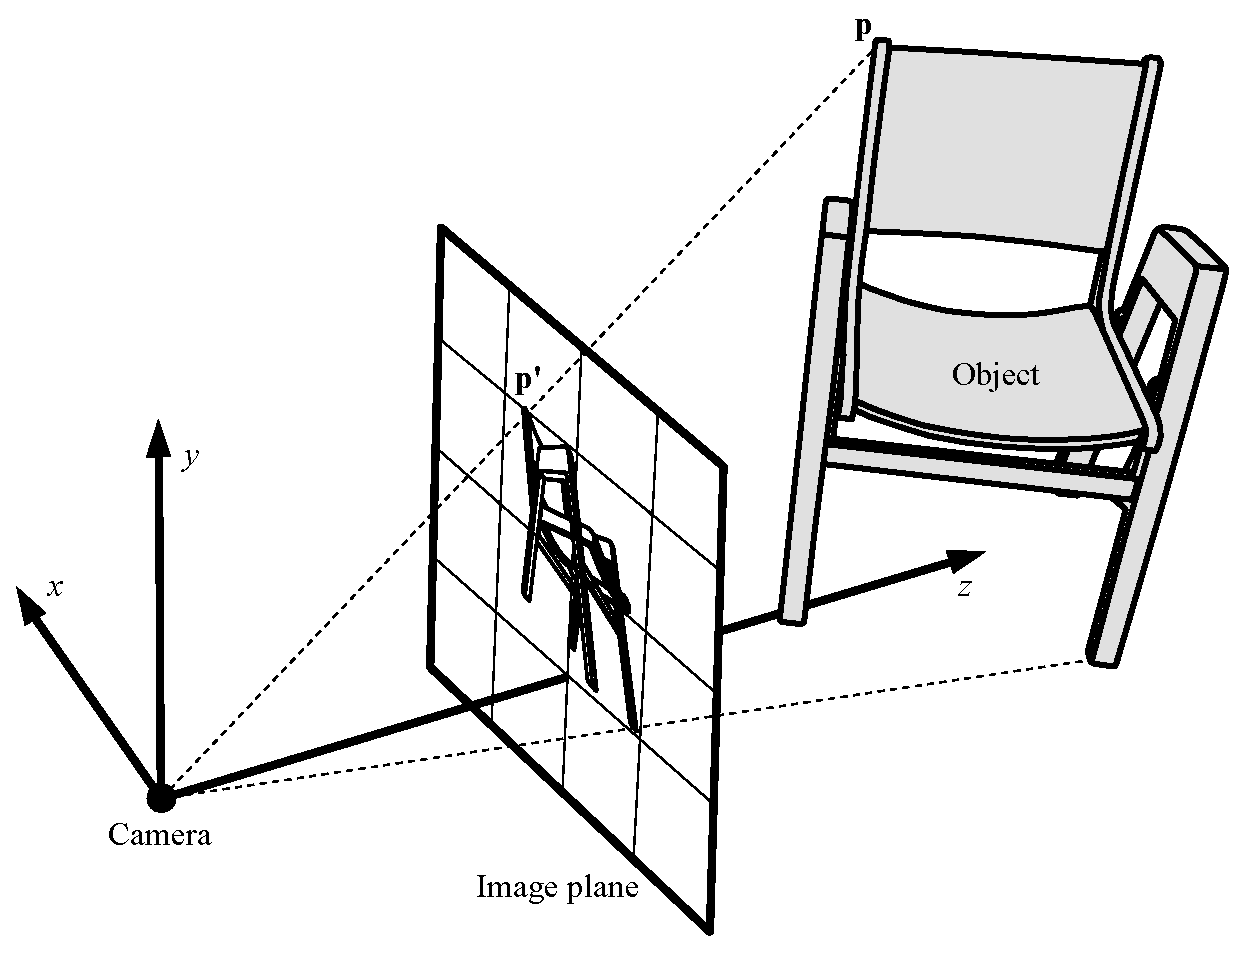
\includegraphics[width=0.90\textwidth]{figures/perspective-chair}
\end{equation*}

% ----------------------------------------------------------------------
\subsection*{Object coordinates}

It is convenient to describe each object in its own coordinate system,
called the \textbf{object coordinate system}%
\index{object coordinates}%
\index{coordinate system!object coordinates}. To illustrate this
concept, we will consider a cube of side length 2, centered at the
origin. The 8 corners of this cube have the following coordinates in
the object coordinate system:
\begin{equation*}
  \begin{mymatrix}{r}  1 \\  1 \\  1 \end{mymatrix},~
  \begin{mymatrix}{r}  1 \\  1 \\ -1 \end{mymatrix},~
  \begin{mymatrix}{r}  1 \\ -1 \\  1 \end{mymatrix},~
  \begin{mymatrix}{r}  1 \\ -1 \\ -1 \end{mymatrix},~
  \begin{mymatrix}{r} -1 \\  1 \\  1 \end{mymatrix},~
  \begin{mymatrix}{r} -1 \\  1 \\ -1 \end{mymatrix},~
  \begin{mymatrix}{r} -1 \\ -1 \\  1 \end{mymatrix},~
  \begin{mymatrix}{r} -1 \\ -1 \\ -1 \end{mymatrix}.
\end{equation*}
For later reference, let us call this the \textbf{standard cube}%
\index{standard cube}. The following picture shows the standard cube
within its object coordinate system:
\begin{equation*}
  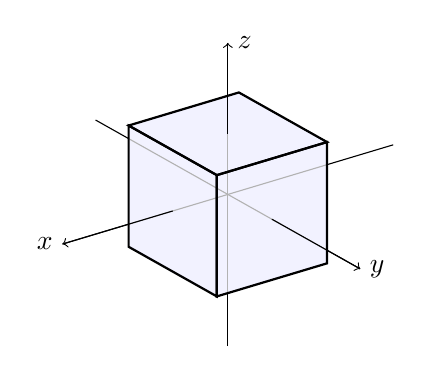
\begin{tikzpicture}[x={(0.8cm,-0.45cm)},y={(1cm,0.3cm)},z={(0cm,1.1cm)},scale=0.7]
    \draw[->] (-3,0,0) -- (3,0,0) node[right]{$y$};
    \draw[->] (0,3,0) -- (0,-3,0) node[left]{$x$};
    \draw[->] (0,0,-2.5) -- (0,0,2.5) node[right]{$z$};
    \begin{scope}
      \clip (1,1,1) -- (1,1,-1) -- (1,-1,-1) -- (-1,-1,-1)
      -- (-1,-1,1) -- (-1,1,1) -- cycle;
      \fill[blue!5] (1,1,1) -- (1,1,-1) -- (1,-1,-1) -- (-1,-1,-1)
      -- (-1,-1,1) -- (-1,1,1) -- cycle;
      \draw[black!30,->] (-3,0,0) -- (3,0,0);
      \draw[black!30,->] (0,-3,0) -- (0,3,0);
      \draw[black!30,->] (0,0,-2.5) -- (0,0,2.5);
    \end{scope}
    \draw[thick] ( 1, 1, 1) -- ( 1, 1,-1) -- ( 1,-1,-1) -- ( 1,-1, 1) -- cycle;
    \draw[thick] ( 1,-1, 1) -- (-1,-1, 1) -- (-1,-1,-1) -- ( 1,-1,-1) -- cycle;
    \draw[thick] ( 1, 1, 1) -- ( 1,-1, 1) -- (-1,-1, 1) -- (-1, 1, 1) -- cycle;
    \draw (1,0,0) -- (3,0,0);
    \draw (0,-3,0) -- (0,-1,0);
    \draw (0,0,1) -- (0,0,2.5);
  \end{tikzpicture}
\end{equation*}

% ----------------------------------------------------------------------
\subsection*{Conversion to camera coordinates}

Before we render an object, we need to place it in some appropriate
location relative to the camera. We do this by specifying four vectors
$\vect{q}$, $\vect{a}_x$, $\vect{a}_y$, and $\vect{a}_z$ in
$\R^3$. Here, $\vect{q}$ is the origin of the object coordinate
system, relative to the camera coordinate system. The vectors
$\vect{a}_x$, $\vect{a}_y$, and $\vect{a}_z$ are the axes of the
object coordinate system, relative to the camera coordinate system, as
shown in the following illustration:
\begin{equation*}
  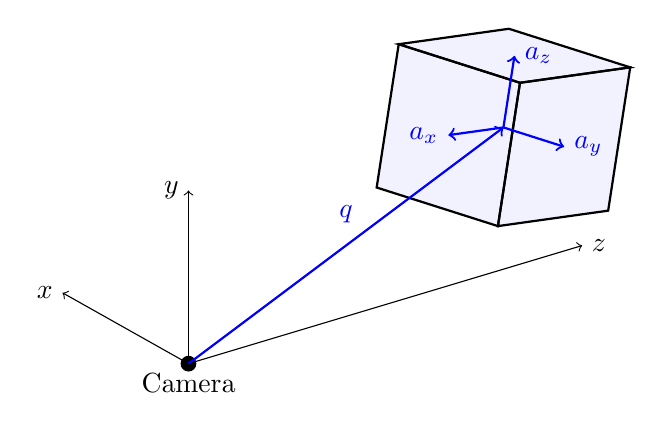
\begin{tikzpicture}
    \fill (0,0) circle (0.1) node[below] {Camera};
    \begin{scope}[x={(-0.8cm,0.45cm)},z={(1cm,0.3cm)},y={(0cm,1.1cm)}]
      \draw[->] (0,0,0) -- (2,0,0) node[left]{$x$};
      \draw[->] (0,0,0) -- (0,2,0) node[left]{$y$};
      \draw[->] (0,0,0) -- (0,0,5) node[right]{$z$};
    \end{scope}
    \begin{scope}[shift={(4,3)}]
      \begin{scope}[x={(-1cm,-0.14cm)},y={(1.1cm,-0.35cm)},z={(0.2cm,1.3cm)},scale=0.7]
        \begin{scope}
          \clip (1,-1,1) -- (1,-1,-1) -- (1,1,-1) -- (-1,1,-1)
          -- (-1,1,1) -- (-1,-1,1) -- cycle;
          \fill[blue!5] (1,-1,1) -- (1,-1,-1) -- (1,1,-1) -- (-1,1,-1)
          -- (-1,1,1) -- (-1,-1,1) -- cycle;
        \end{scope}
        \draw[thick] ( 1, 1, 1) -- ( 1, 1,-1) -- ( 1,-1,-1) -- ( 1,-1, 1) -- cycle;
        \draw[thick] ( 1, 1, 1) -- (-1, 1, 1) -- (-1, 1,-1) -- ( 1, 1,-1) -- cycle;
        \draw[thick] ( 1, 1, 1) -- ( 1,-1, 1) -- (-1,-1, 1) -- (-1, 1, 1) -- cycle;
        \draw[thick,blue,->] (0,0,0) -- (1,0,0) node[left]{$\vect{a}_x$};
        \draw[thick,blue,->] (0,0,0) -- (0,1,0) node[right]{$\vect{a}_y$};
        \draw[thick,blue,->] (0,0,0) -- (0,0,1) node[right]{$\vect{a}_z$};
      \end{scope}
    \end{scope}
    \draw[thick,blue,->] (0,0) -- node[above=1ex]{$\vect{q}$}(4,3);
  \end{tikzpicture}
\end{equation*}
Thus, given a point with object coordinates
$\vect{v}=\begin{mymatrix}{c}x\\y\\z\end{mymatrix}$, we can find its
camera coordinates
$\vect{p} = \begin{mymatrix}{c} p_x \\ p_y \\ p_z \end{mymatrix}$ by
the following formula:
\begin{equation*}
  \vect{p} = \vect{q} + x\vect{a}_x + y\vect{a}_y + z\vect{a}_z.
\end{equation*}
If we write $A$ for the $3\times 3$-matrix whose columns are $\vect{a}_x$,
$\vect{a}_y$, and $\vect{a}_z$, we can also write this formula more succinctly as
\begin{equation*}
  \vect{p} = \vect{q} + A\vect{v}.
\end{equation*}

\begin{example}{Converting object coordinates to camera coordinates}{object-to-camera}
  Let
  \begin{equation*}
    \vect{q} = \begin{mymatrix}{c} 0 \\ 0.5 \\ 5 \end{mymatrix},\quad
    A = \begin{mymatrix}{ccc}
      0.8 & 0.6 & 0 \\
      0 & 0 & 1 \\
      0.6 & -0.8 & 0 \\
    \end{mymatrix}.
  \end{equation*}
  Convert each of the 8 corners of the standard cube from object
  coordinates to camera coordinates.
\end{example}

\begin{solution}
  Let $\vect{v}_1,\ldots,\vect{v}_8$ be the object coordinates of the
  8 corners of the cube:
  \begin{equation*}
    \begin{mymatrix}{r}  1 \\  1 \\  1 \end{mymatrix},~
    \begin{mymatrix}{r}  1 \\  1 \\ -1 \end{mymatrix},~
    \begin{mymatrix}{r}  1 \\ -1 \\  1 \end{mymatrix},~
    \begin{mymatrix}{r}  1 \\ -1 \\ -1 \end{mymatrix},~
    \begin{mymatrix}{r} -1 \\  1 \\  1 \end{mymatrix},~
    \begin{mymatrix}{r} -1 \\  1 \\ -1 \end{mymatrix},~
    \begin{mymatrix}{r} -1 \\ -1 \\  1 \end{mymatrix},~
    \begin{mymatrix}{r} -1 \\ -1 \\ -1 \end{mymatrix}.
  \end{equation*}
  We convert each of them to camera coordinates using the formula
  $\vect{p}_i = \vect{q} + A\vect{v}_i$:
  \begin{eqnarray*}
    \vect{p}_1 &=&
    \begin{mymatrix}{c} 0 \\ 0.5 \\ 5 \end{mymatrix}
    + \begin{mymatrix}{ccc}
      0.8 & 0.6 & 0 \\
      0 & 0 & 1 \\
      0.6 & -0.8 & 0 \\
    \end{mymatrix}
    \begin{mymatrix}{r}  1 \\  1 \\  1 \end{mymatrix}
    ~=~
    \begin{mymatrix}{r}  1.4 \\  1.5 \\ 4.8 \end{mymatrix}, \\
    \vect{p}_2 &=&
    \begin{mymatrix}{c} 0 \\ 0.5 \\ 5 \end{mymatrix}
    + \begin{mymatrix}{ccc}
      0.8 & 0.6 & 0 \\
      0 & 0 & 1 \\
      0.6 & -0.8 & 0 \\
    \end{mymatrix}
    \begin{mymatrix}{r}  1 \\  1 \\ -1 \end{mymatrix}
    ~=~
    \begin{mymatrix}{r}  1.4 \\ -0.5 \\ 4.8 \end{mymatrix}, \\
    \vect{p}_3 &=&
    \begin{mymatrix}{c} 0 \\ 0.5 \\ 5 \end{mymatrix}
    + \begin{mymatrix}{ccc}
      0.8 & 0.6 & 0 \\
      0 & 0 & 1 \\
      0.6 & -0.8 & 0 \\
    \end{mymatrix}
    \begin{mymatrix}{r}  1 \\ -1 \\ 1 \end{mymatrix}
    ~=~
    \begin{mymatrix}{r}  0.2 \\ 1.5 \\ 6.4 \end{mymatrix}, \\
  \end{eqnarray*}
  and so on. Continuing in the same fashion, we find
  $\vect{p}_1,\ldots,\vect{p}_8$:
  \begin{equation}\label{eqn:object-to-camera}
    \begin{mymatrix}{r}  1.4 \\  1.5 \\ 4.8 \end{mymatrix},
    \begin{mymatrix}{r}  1.4 \\ -0.5 \\ 4.8 \end{mymatrix},
    \begin{mymatrix}{r}  0.2 \\  1.5 \\ 6.4 \end{mymatrix},
    \begin{mymatrix}{r}  0.2 \\ -0.5 \\ 6.4 \end{mymatrix},
    \begin{mymatrix}{r} -0.2 \\  1.5 \\ 3.6 \end{mymatrix},
    \begin{mymatrix}{r} -0.2 \\ -0.5 \\ 3.6 \end{mymatrix},
    \begin{mymatrix}{r} -1.4 \\  1.5 \\ 5.2 \end{mymatrix},
    \begin{mymatrix}{r} -1.4 \\ -0.5 \\ 5.2 \end{mymatrix}.
  \end{equation}
\end{solution}

We can also write $f:\R^3 \to \R^3$ for the function that converts
object coordinates to camera coordinates, i.e.,
\begin{equation*}
  f(\vect{v}) = \vect{q} + A\vect{v}.
\end{equation*}
We note that this is not a linear function, because
$f(\vect{0})\neq \vect{0}$. The function $f$ is called an
\textbf{affine function}%
\index{function!affine}%
\index{affine function}, which means that it is a linear function
$\vect{v}\mapsto A\vect{v}$ followed by a translation
$\vect{v}\mapsto \vect{q}+\vect{v}$.

% ----------------------------------------------------------------------
\subsection*{Rendering}

Once we know the camera coordinates
$\vect{p}=\begin{mymatrix}{c} p_x \\ p_y \\ p_z \end{mymatrix}$ of a point,
we need to render the point, i.e., find its coordinates in the image plane.
\begin{equation*}
  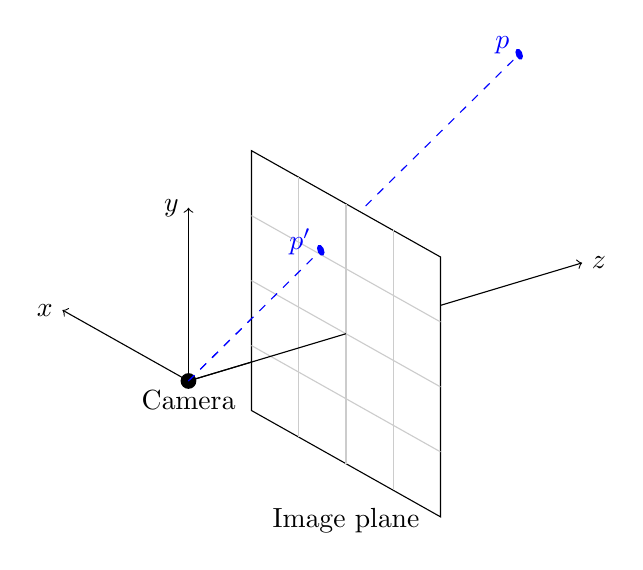
\begin{tikzpicture}
    \fill (0,0) circle (0.1) node[below] {Camera};
    \begin{scope}[x={(-0.8cm,0.45cm)},z={(1cm,0.3cm)},y={(0cm,1.1cm)}]
      \draw[->] (0,0,0) -- (2,0,0) node[left]{$x$};
      \draw[->] (0,0,0) -- (0,2,0) node[left]{$y$};
      \draw[->] (0,0,0) -- (0,0,5) node[right]{$z$};
      \draw[dashed,blue] (0,0,0) -- (1,2,5);
      \draw[fill=white] (-1.5,-1.5,2) -- (-1.5,1.5,2) -- (1.5,1.5,2) -- (1.5,-1.5,2) -- cycle;
      \draw[thin,black!20] (-1.5,-0.75,2) -- (1.5,-0.75,2);
      \draw[thin,black!20] (-1.5,0,2) -- (1.5,0,2);
      \draw[thin,black!20] (-1.5,0.75,2) -- (1.5,0.75,2);
      \draw[thin,black!20] (-0.75,-1.5,2) -- (-0.75,1.5,2);
      \draw[thin,black!20] (0,-1.5,2) -- (0,1.5,2);
      \draw[thin,black!20] (0.75,-1.5,2) -- (0.75,1.5,2);
      \fill[blue] (1,2,5) circle (0.06) +(0,0.1,0) node[left] {$\vect{p}$};
      \fill[blue] (0.4,0.8,2) circle (0.06) +(0,0.1,0) node[left] {$\vect{p}'$};
      \draw (0,0,0) -- (0,0,2);
      \draw[dashed,blue] (0,0,0) -- (0.4,0.8,2);
      \path (0,-1.9,2) node[below] {Image plane};
    \end{scope}
  \end{tikzpicture}
\end{equation*}
Since the camera is located at the origin, the line that passes
through the camera and the point $\vect{p}$ has the parametric equation
\begin{equation*}
  \vect{r} = t\vect{p} = \begin{mymatrix}{c} tp_x \\ tp_y \\ tp_z \end{mymatrix}.
\end{equation*}
Since the image plane is the plane $z=1$, we must set $t$ such that
$tp_z = 1$, i.e., $t=\frac{1}{p_z}$. Therefore, the coordinates of the
rendered point are
\begin{equation*}
  \vect{p}' = \frac{1}{p_z}\vect{p} =
  \begin{mymatrix}{c} p_x/p_z \\ p_y/p_z \\ 1 \end{mymatrix}.
\end{equation*}
Finally, since the image plane is $2$-dimensional, we can forget the
now useless $z$-coordinate, and render the point at the coordinates
$\begin{mymatrix}{c} p_x/p_z \\ p_y/p_z \end{mymatrix}$ in the
$2$-dimensional image plane.

\begin{example}{Rendering}{rendering}
  Render the cube from Example~\ref{exa:object-to-camera}.
\end{example}

\begin{solution}
  We must apply the rendering function
  \begin{equation*}
    g\paren{\begin{mymatrix}{c} p_x \\ p_y \\ p_z \end{mymatrix}}
    = \begin{mymatrix}{c} p_x/p_z \\ p_y/p_z \end{mymatrix}
  \end{equation*}
  to each of the corners of the cube from
  {\eqref{eqn:object-to-camera}}.
  We have
  \begin{eqnarray*}
    g\paren{\begin{mymatrix}{r}  1.4 \\  1.5 \\ 4.8 \end{mymatrix}}
    &=& \begin{mymatrix}{r} 1.4/4.8 \\ 1.5/4.8 \end{mymatrix}
    ~=~ \begin{mymatrix}{r} 0.292 \\ 0.312 \end{mymatrix}, \\
    g\paren{\begin{mymatrix}{r}  1.4 \\ -0.5 \\ 4.8 \end{mymatrix}}
    &=& \begin{mymatrix}{r} 1.4/4.8 \\ -0.5/4.8 \end{mymatrix}
    ~=~ \begin{mymatrix}{r} 0.292 \\ -0.104 \end{mymatrix}, \\
    g\paren{\begin{mymatrix}{r}  0.2 \\  1.5 \\ 6.4 \end{mymatrix}}
    &=& \begin{mymatrix}{r} 0.2/6.4 \\ 1.5/6.4 \end{mymatrix}
    ~=~ \begin{mymatrix}{r} 0.031 \\ 0.234 \end{mymatrix}, \\
  \end{eqnarray*}
  and so on. The 8 rendered points are:
  \begin{equation*}
    \begin{mymatrix}{r} 0.292 \\ 0.312 \end{mymatrix},~
    \begin{mymatrix}{r} 0.292 \\ -0.104 \end{mymatrix},~
    \begin{mymatrix}{r} 0.031 \\ 0.234 \end{mymatrix},~
    \begin{mymatrix}{r} 0.031 \\ -0.078 \end{mymatrix},~
    \begin{mymatrix}{r} -0.056 \\ 0.417 \end{mymatrix},~
    \begin{mymatrix}{r} -0.056 \\ -0.139 \end{mymatrix},~
    \begin{mymatrix}{r} -0.269 \\ 0.288 \end{mymatrix},~
    \begin{mymatrix}{r} -0.269 \\ -0.096 \end{mymatrix}.
  \end{equation*}
  Drawing these in the 2-dimensional image plane, we get the following
  picture, which is the final perspective-rendered image of the cube:
  \begin{equation*}
    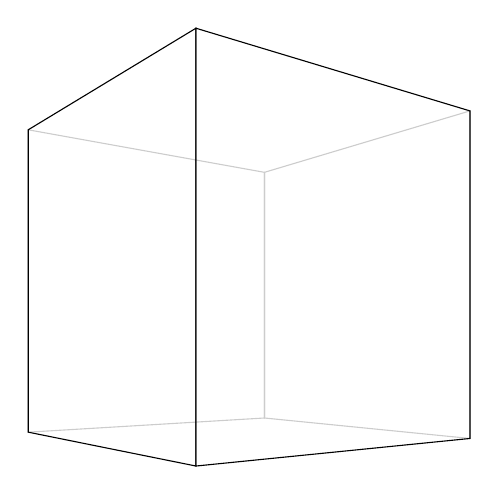
\begin{tikzpicture}[scale=10]
      \draw[black!20] (0.292,0.312) -- (0.292,-0.104) -- (0.031,-0.078) -- (0.031,0.234) -- cycle;
      \draw[black!20] (0.031,0.234) -- (0.031,-0.078) -- (-0.269,-0.096) -- (-0.269,0.288) -- cycle;
      \draw (-0.056,0.417) -- (-0.056,-0.139) -- (-0.269,-0.096) -- (-0.269,0.288) -- cycle;
      \draw (0.292,0.312) -- (0.292,-0.104) -- (-0.056,-0.139) -- (-0.056,0.417) -- cycle;
    \end{tikzpicture}
  \end{equation*}
\end{solution}

% ----------------------------------------------------------------------
\subsection*{Animation}

We placed our object in the camera coordinate system using a
coordinate transformation function
\begin{equation*}
  f(\vect{v}) = \vect{q} + A\vect{v}.
\end{equation*}
One of the advantages of using such a coordinate transformation (as
opposed to specifying the object points directly in the camera
coordinate system) is that this makes it very easy to move the objects
around, rotate them, scale and shrink them, etc. For example:
\begin{enumerate}
\item To move the object to a different location, we only have to
  change the vector $\vect{q}$.
\item To rotate the object about its own $z$-axis, we only have to
  replace $\vect{v}$ by $R_{\theta}\vect{v}$, where $R_{\theta}$ is the matrix for a
  rotation about the $z$-axis by angle $\theta$:
  \begin{equation*}
    R_{\theta} = \begin{mymatrix}{ccc}
      \cos\theta & -\sin\theta & 0 \\
      \sin\theta & \cos\theta & 0 \\
      0 & 0 & 1 \\
    \end{mymatrix}.
  \end{equation*}
\end{enumerate}
Similarly tp $R_{\theta}$, we can also insert other transformation
matrices (for example, we could rotate the object about its $x$-axis
instead of its $z$-axis, scale the object, etc).  We can even make an
animation by rendering the object repeatedly for different values of
these parameters.

\begin{example}{An animated cube}{animation}
  Make an animation of a rotating, moving cube. The animation is 5
  seconds long (i.e., time $t$ ranges from $0$ to $5$). The location
  of the cube at time $t$, in camera coordinates, is given by
  \begin{equation*}
    \vect{q}(t) =
    \begin{mymatrix}{c} -3+3t \\ -3 \\ 8+3t \end{mymatrix}.
  \end{equation*}
  The transformation matrix $A$ is as in
  Example~\ref{exa:object-to-camera}. Moreover, the cube should make
  one quarter rotation about its $z$-axis during the time of the
  animation, i.e., it should be transformed by $R_{\theta}$, where
  $\theta=\frac{\pi}{10}t$. Compute $6$ frames of the animation, for
  $t=0$, $t=1$, \ldots, $t=5$.
\end{example}

\begin{solution}
  For each of the animation frames $t\in\set{0,1,2,3,4,5}$, we do a
  calculation very similar to that of
  Examples~\ref{exa:object-to-camera} to convert the cube coordinates
  to camera coordinates, using the coordinate transformation
  \begin{equation*}
    f(\vect{v}) = \vect{q}(t) + AR_{\theta}\vect{v},
  \end{equation*}
  where $\theta=\frac{\pi}{10}t$. We then render each of the frames
  using the same method as in Example~\ref{exa:rendering}. We skip the
  detailed calculations, which are best done by computer (though they
  could be done by hand, of course, as we did in
  Examples~\ref{exa:object-to-camera} and {\ref{exa:rendering}}. The
  final rendered frames look like this:
  \begin{equation*}
    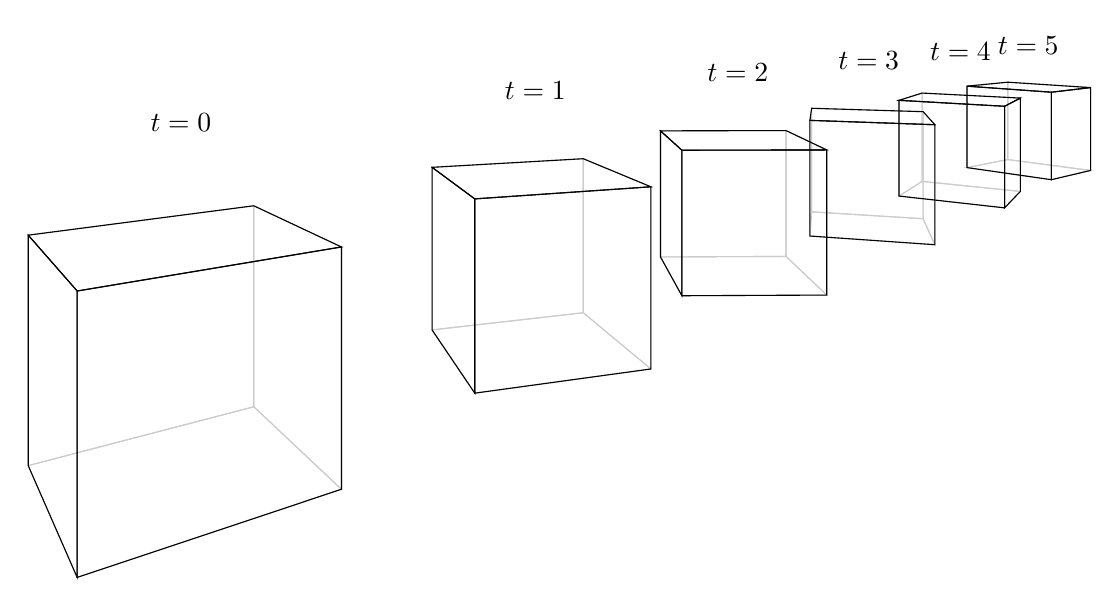
\begin{tikzpicture}[scale=12]
      % Background:
      \draw[black!20] (-0.2979,-0.2128) -- (-0.5366,-0.2439) -- (-0.5366,-0.4878) -- (-0.2979,-0.4255) -- cycle;
      \draw[black!20] (-0.2051,-0.5128) -- (-0.2979,-0.4255) -- (-0.5366,-0.4878) -- (-0.4848,-0.6061) -- cycle;
      \draw[black!20] (-0.2051,-0.2564) -- (-0.2979,-0.2128) -- (-0.2979,-0.4255) -- (-0.2051,-0.5128) -- cycle;
      
      \draw[black!20] (0.0508,-0.1630) -- (-0.1092,-0.1721) -- (-0.1092,-0.3442) -- (0.0508,-0.3260) -- cycle;
      \draw[black!20] (0.1224,-0.3855) -- (0.0508,-0.3260) -- (-0.1092,-0.3442) -- (-0.0640,-0.4111) -- cycle;
      \draw[black!20] (0.1224,-0.1927) -- (0.0508,-0.1630) -- (0.0508,-0.3260) -- (0.1224,-0.3855) -- cycle;
      
      \draw[black!20] (0.2654,-0.1332) -- (0.1325,-0.1335) -- (0.1325,-0.2669) -- (0.2654,-0.2664) -- cycle;
      \draw[black!20] (0.3085,-0.3073) -- (0.2654,-0.2664) -- (0.1325,-0.2669) -- (0.1552,-0.3080) -- cycle;
      \draw[black!20] (0.3085,-0.1537) -- (0.2654,-0.1332) -- (0.2654,-0.2664) -- (0.3085,-0.3073) -- cycle;

      \draw[black!20] (0.2907,-0.1224) -- (0.2907,-0.2448) -- (0.2925,-0.2192) -- (0.2925,-0.1096) -- cycle;
      \draw[black!20] (0.4105,-0.1132) -- (0.2925,-0.1096) -- (0.2925,-0.2192) -- (0.4105,-0.2265) -- cycle;
      \draw[black!20] (0.4229,-0.2540) -- (0.4105,-0.2265) -- (0.2925,-0.2192) -- (0.2907,-0.2448) -- cycle;
      \draw[black!20] (0.4229,-0.1270) -- (0.4105,-0.1132) -- (0.4105,-0.2265) -- (0.4229,-0.2540) -- cycle;

      \draw[black!20] (0.3850,-0.1012) -- (0.3850,-0.2025) -- (0.4094,-0.1870) -- (0.4094,-0.0935) -- cycle;
      \draw[black!20] (0.5134,-0.0988) -- (0.4094,-0.0935) -- (0.4094,-0.1870) -- (0.5134,-0.1976) -- cycle;
      \draw[black!20] (0.4967,-0.2150) -- (0.5134,-0.1976) -- (0.4094,-0.1870) -- (0.3850,-0.2025) -- cycle;

      \draw[black!20] (0.4569,-0.0862) -- (0.4569,-0.1724) -- (0.5000,-0.1639) -- (0.5000,-0.0820) -- cycle;
      \draw[black!20] (0.5877,-0.0877) -- (0.5000,-0.0820) -- (0.5000,-0.1639) -- (0.5877,-0.1754) -- cycle;
      \draw[black!20] (0.5463,-0.1852) -- (0.5877,-0.1754) -- (0.5000,-0.1639) -- (0.4569,-0.1724) -- cycle;

      % Foreground:
      \draw (-0.4848,-0.3030) -- (-0.4848,-0.6061) -- (-0.5366,-0.4878) -- (-0.5366,-0.2439) -- cycle;
      \draw (-0.2051,-0.2564) -- (-0.2051,-0.5128) -- (-0.4848,-0.6061) -- (-0.4848,-0.3030) -- cycle;
      \draw (-0.2051,-0.2564) -- (-0.4848,-0.3030) -- (-0.5366,-0.2439) -- (-0.2979,-0.2128) -- cycle;

      \draw (-0.0640,-0.2055) -- (-0.0640,-0.4111) -- (-0.1092,-0.3442) -- (-0.1092,-0.1721) -- cycle;
      \draw (0.1224,-0.1927) -- (0.1224,-0.3855) -- (-0.0640,-0.4111) -- (-0.0640,-0.2055) -- cycle;
      \draw (0.1224,-0.1927) -- (-0.0640,-0.2055) -- (-0.1092,-0.1721) -- (0.0508,-0.1630) -- cycle;

      \draw (0.1552,-0.1540) -- (0.1552,-0.3080) -- (0.1325,-0.2669) -- (0.1325,-0.1335) -- cycle;
      \draw (0.3085,-0.1537) -- (0.3085,-0.3073) -- (0.1552,-0.3080) -- (0.1552,-0.1540) -- cycle;
      \draw (0.3085,-0.1537) -- (0.1552,-0.1540) -- (0.1325,-0.1335) -- (0.2654,-0.1332) -- cycle;

      \draw (0.4229,-0.1270) -- (0.4229,-0.2540) -- (0.2907,-0.2448) -- (0.2907,-0.1224) -- cycle;
      \draw (0.4229,-0.1270) -- (0.2907,-0.1224) -- (0.2925,-0.1096) -- (0.4105,-0.1132) -- cycle;

      \draw (0.4967,-0.1075) -- (0.5134,-0.0988) -- (0.5134,-0.1976) -- (0.4967,-0.2150) -- cycle;
      \draw (0.4967,-0.1075) -- (0.4967,-0.2150) -- (0.3850,-0.2025) -- (0.3850,-0.1012) -- cycle;
      \draw (0.4967,-0.1075) -- (0.3850,-0.1012) -- (0.4094,-0.0935) -- (0.5134,-0.0988) -- cycle;

      \draw (0.5463,-0.0926) -- (0.5877,-0.0877) -- (0.5877,-0.1754) -- (0.5463,-0.1852) -- cycle;
      \draw (0.5463,-0.0926) -- (0.5463,-0.1852) -- (0.4569,-0.1724) -- (0.4569,-0.0862) -- cycle;
      \draw (0.5463,-0.0926) -- (0.4569,-0.0862) -- (0.5000,-0.0820) -- (0.5877,-0.0877) -- cycle;

      % Labels:
      \path (-0.3750,-0.1250) node {$t=0$};
      \path (0.0000,-0.0909) node {$t=1$};
      \path (0.2143,-0.0714) node {$t=2$};
      \path (0.3529,-0.0588) node {$t=3$};
      \path (0.4500,-0.0500) node {$t=4$};
      \path (0.5217,-0.0435) node {$t=5$};
    \end{tikzpicture}
  \end{equation*}
  Note that there is a bit of distortion in the first and last cubes.
  This is because the camera is very close to the image plane (the
  scene has been ``filmed'' with a wide-angle camera). The distortion
  goes away if you close one eye and bring the other one to about 10cm
  from the page.
\end{solution}
